%%%%%%%%%%%%%%%%%%%%%%%%%%%%%%%%%%%%%%%%%%%%%%%%%%%%%%%%%%%%%%%%%%%%%%%%%%%%%%%%%%
\begin{frame}[fragile]\frametitle{}
\begin{center}
{\Large Linear Regression - Advertising Budget Example}
\end{center}
\end{frame}

%%%%%%%%%%%%%%%%%%%%%%%%%%%%%%%%%%%%%%%%%%%%%%%%%%%%%%%%%%%%%%%%%%%%%%%%
\begin{frame}[fragile]\frametitle{Example: Advertising Dataset}
\begin{itemize}
\item Toy Dataset: Advertising, Advertising.csv 
\item Sales totals for a product in 200 different markets. Advertising budget in each market, broken down into TV, radio, newspaper
\end{itemize}
%\begin{lstlisting}
%import pandas as pd
%advertising = pd.read_csv('../datasets/Advertising.csv')
%advertising.head(5)
%\end{lstlisting}
\begin{center}

\includegraphics[width=0.8\linewidth]{advtdata}
\end{center}
({\small Data: https://www.statlearning.com)}
\end{frame}


%%%%%%%%%%%%%%%%%%%%%%%%%%%%%%%%%%%%%%%%%%%%%%%%%%%%%%%%%%%%%%%%%%%%%%%%
\begin{frame}[fragile]\frametitle{Problem}
\begin{itemize}
\item Goal: What marketing plan for next year will result in high product sales?
\item Questions (Hypothesis):
	\begin{itemize}
	\item Is there a relationship between advertising budgets and sales?
	\item How strong is the relationship between advertising budgets and sales?
	\item Which media contribute to the sales the most?
%	\item How accurately can we estimate the effect of each medium on sales?
	\item Is the relationship linear?
%	\item Is there any interaction effect? (called ``synergy'' in business). Example: spending 50k on TV ads + 50k on radio ads results in more sales than spending 100k on only TV
	\end{itemize}
\end{itemize}
\end{frame}


%%%%%%%%%%%%%%%%%%%%%%%%%%%%%%%%%%%%%%%%%%%%%%%%%%%%%%%%%%%%%%%%%%%%%%%%
\begin{frame}[fragile]\frametitle{EDA: the Correlation Matrix}
Correlation Matrix

\begin{center}

\includegraphics[width=0.8\linewidth]{corrmat}
\end{center}
\begin{itemize}
\item Correlation between radio and newspaper is 0.35
\item Barely any correlation (or ``not correlated'') for TV/radio and TV/newspaper
\end{itemize}
\end{frame}

%%%%%%%%%%%%%%%%%%%%%%%%%%%%%%%%%%%%%%%%%%%%%%%%%%%%%%%%%%%%%%%%%%%%%%%%
\begin{frame}[fragile]\frametitle{EDA: Reading the Correlation Matrix}
\begin{center}

\includegraphics[width=0.8\linewidth]{corrmat}
\end{center}
\begin{itemize}
\item Reveals tendency to spend more on Newspaper advertising in markets where more is spent on Radio advertising.
\item Sales higher in markets where more is spent on Radio, but more also tends to be spent on Newspaper.
\item In simple linear regression: Newspaper ``gets credit'' for effect of Radio on Sales.
\end{itemize}
\end{frame}
%%%%%%%%%%%%%%%%%%%%%%%%%%%%%%%%%%%%%%%%%%%%%%%%%%%%%%%%%%%%%%%%%%%%%%%%
\begin{frame}[fragile]\frametitle{Advertising Dataset: Regressing Sales on TV}
\begin{itemize}
\item What are some ways we can regress sales onto advertising using Simple Linear Regression?
\item One model:

\begin{align*}
sales &\approx \beta_0 + \beta_1 \times TV \\
y &\approx \beta_0 + \beta_1 \times x
\end{align*}

\item Scatter plot visualization for TV and Sales.
%\begin{lstlisting}
%%matplotlib inline
%advertising.plot.scatter(x='TV', y='Sales');
%\end{lstlisting}
\begin{center}

\includegraphics[width=0.4\linewidth]{advtscatter}
\end{center}
\end{itemize}
\end{frame}

%%%%%%%%%%%%%%%%%%%%%%%%%%%%%%%%%%%%%%%%%%%%%%%%%%%%%%%%%%%%%%%%%%%%%%%%
\begin{frame}[fragile]\frametitle{Advertising Dataset: the Fitted Line}
\begin{itemize}
\item Simple Linear Model in Python (using pandas and scikit): Predictor: $x$, Response: $y$
%\begin{lstlisting}
%reg = linear_model.LinearRegression()
%reg.fit(advertising['TV'].reshape(-1,1), advertising['Sales'].reshape(-1,1))
%print('Coefficients: \n', reg.coef_)
%print('Intercept: \n', reg.intercept_)
%
%Coefficients: [[ 0.04753664]] 
%Intercept: [ 7.03259355]
%\end{lstlisting}
\item $Sales = 7.03259 + 0.04754  \times  TV$
\end{itemize}
\end{frame}

%%%%%%%%%%%%%%%%%%%%%%%%%%%%%%%%%%%%%%%%%%%%%%%%%%%%%%%%%%%%%%%%%%%%%%%%
\begin{frame}[fragile]\frametitle{Advertising Dataset: Can We Combine Three Models?}
Scatter plot visualization for TV and Sales with Linear Model.
%\begin{lstlisting}
%plt.scatter(advertising['TV'], advertising['Sales'],  color='black')
%plt.plot(advertising['TV'], reg.predict(advertising['TV'].reshape(-1,1)), 
%         color='blue', linewidth=3)
%
%\end{lstlisting}
\begin{center}

\includegraphics[width=0.6\linewidth]{advtscatterline}
\end{center}

If we have 3 such models, can we ``somehow'' compose them (say, averaging) to get the combined model?

\end{frame}

%
%%%%%%%%%%%%%%%%%%%%%%%%%%%%%%%%%%%%%%%%%%%%%%%%%%%%%%%%%%%%%%%%%%%%%%%%%
%\begin{frame}[fragile]\frametitle{Quality}
%Measuring the Quality of a Regression Model. Residual Standard Error
%\begin{array}
%RSE = \sqrt{\frac{RSS}{(n-2)}}
%\end{array}
%Advertising Dataset
%$RSE = 3.2586563 \approx 3.25$
%Confidence Interval for the Mean Value of $y$ given $x$
%\begin{center}
%
\includegraphics[width=0.4\linewidth]{advtconf}
%\end{center}
%\end{frame}
%
%
%%%%%%%%%%%%%%%%%%%%%%%%%%%%%%%%%%%%%%%%%%%%%%%%%%%%%%%%%%%%%%%%%%%%%%%%%
%\begin{frame}[fragile]\frametitle{Comparison: Confidence Interval vs. Prediction Interval}
%Analogy
%\begin{itemize}
%\item Trying to predict baseball batting average
%\item ``Team'' batting averages (mean of the player batting averages on that team), for all 30 teams, have low variance. Should be easier to predict a team batting average
%\item ``Individual batting averages are quite varied (some players are good, while some players are Ryan Howard). Estimate of team average will be more precise than an estimate of a randomly chosen player, for the same level of confidence
%\end{itemize}
%\end{frame}
%
%%%%%%%%%%%%%%%%%%%%%%%%%%%%%%%%%%%%%%%%%%%%%%%%%%%%%%%%%%%%%%%%%%%%%%%%%
%\begin{frame}[fragile]\frametitle{Evaluating using a Test Set}
%%Given a set of predictions for m new cases, we can evaluate the model's predictions by
%\begin{itemize}
%\item Mean Error (ME): should be close to zero
%\begin{center}
%
\includegraphics[width=0.4\linewidth]{meanerr}
%\end{center}
%%\item Residual Standard Error:$RSE = \sqrt{\frac{RSS}{(n-2)}}$
%\item Root Mean Square Error (RMSE)
%\begin{center}
%
\includegraphics[width=0.4\linewidth]{meanrsqr}
%\end{center}
%%\item Mean Absolute Percent Error (MAPE)
%%\begin{center}
%%
\includegraphics[width=0.4\linewidth]{meanmape}
%%\end{center}
%\end{itemize}
%\end{frame}

%%%%%%%%%%%%%%%%%%%%%%%%%%%%%%%%%%%%%%%%%%%%%%%%%%%%%%%%%%%%%%%%%%%%%%%%%%
%%\begin{frame}[fragile]\frametitle{Advertising Dataset}
%%\begin{itemize}
%%\item RSE = 3.26. Actual sales in each market deviate from the true regression line by approximately 3.26 units, on average.
%%\item Is this error amount acceptable?
%%\item Business answer: depends on problem context
%%\item Worth noting the percentage error:
%%$PercentageError = \frac{RSE}{Mean\_Sales} = \frac{3.26}{14} = 0.23238 = 23\%$
%%\item RSE measures the ``lack of fit'' that a model may have.
%%
%%\end{itemize}
%%\end{frame}





%%%%%%%%%%%%%%%%%%%%%%%%%%%%%%%%%%%%%%%%%%%%%%%%%%%%%%%%%%%%%%%%%%%%%%%%
\begin{frame}[fragile]\frametitle{Multiple Linear Regression}
\begin{itemize}
\item In practice, often have more than one predictor
\begin{itemize}
\item $sales \approx \beta_{0,1} + \beta_{1,1} \times TV$
\item $sales \approx \beta_{0,2} + \beta_{1,2} \times Newspaper$
\item $sales \approx \beta_{0,3} + \beta_{1,3} \times radio$
\end{itemize}
\item Run three separate simple linear regressions
\item For p predictor variables:
$ Y = \beta_0 + \beta_1 X_1 + \beta_2 X_2 + \ldots + \beta_p X_p + \epsilon$
\item Since error $\epsilon$ has mean zero, we usually omit it.
\item A one-unit change in predictor $X_j$ changes the expected response by $\beta_j$ units, holding every other predictor fixed.
\item That last clause is the whole difference from fitting one predictor at a time.
\item For our case:
$ sales = \beta_0 + \beta_1 \times TV + \beta_2 \times radio + \beta_3 \times newspaper$
\end{itemize}
\end{frame}


%%
%%%%%%%%%%%%%%%%%%%%%%%%%%%%%%%%%%%%%%%%%%%%%%%%%%%%%%%%%%%%%%%%%%%%%%%%%%
%%\begin{frame}[fragile]\frametitle{Estimating the Parameters $\beta_0,\beta_1,\ldots$}
%%\begin{itemize}
%%\item Parameters (regression coefficients) are typically estimated through the method of least squares
%%\item Residual Sum of Squares (RSS):
%%\begin{array}
%%RSS &= \sum (y_i - \hat{y_i})^2\\
%%&= \sum (y_i -  \hat{\beta_0} + \hat{\beta_1} X_1 + \hat{\beta_2} X_2 + \ldots + \hat{\beta_p} X_p)^2
%%\end{array}
%%\item We want to minimize the RSS
%%\end{itemize}
%%\end{frame}




%%%%%%%%%%%%%%%%%%%%%%%%%%%%%%%%%%%%%%%%%%%%%%%%%%%%%%%%%%%%%%%%%%%%%%%%
\begin{frame}[fragile]\frametitle{Estimating the Parameters $\beta_0,\beta_1,\ldots$}
\begin{itemize}
\item Advertising Dataset
$ sales = \beta_0 + \beta_1 \times TV + \beta_2 \times radio + \beta_3 \times newspaper$
\item After solving
$ sales = 2.93 + 0.0457 \times TV + 0.188 \times radio - 0.0010 \times newspaper$
\end{itemize}
\end{frame}

%%%%%%%%%%%%%%%%%%%%%%%%%%%%%%%%%%%%%%%%%%%%%%%%%%%%%%%%%%%%%%%%%%%%%%%%
\begin{frame}[fragile]\frametitle{Coefficients}
\begin{itemize}
\item Many Simple Linear Regressions, one per medium (slope, then intercept):
	\begin{itemize}
	\item TV model: slope \texttt{0.04753664}, intercept \texttt{7.03259355}
	\item Radio model: slope \texttt{0.20249578}, intercept \texttt{9.31163810}
	\item Newspaper model: slope \texttt{0.05469310}, intercept \texttt{12.35140707}
%	\item Slope term (newspaper coefficient) represents the average effect of a \$1,000 increase in newspaper advertising, ignoring other predictors (TV and radio).
	\end{itemize}

\item Single Multiple Linear Regression
	\begin{itemize}
	\item Slopes: TV \texttt{0.04576465}, radio \texttt{0.18853002}, newspaper \texttt{-0.00103749}
	\item Intercept: \texttt{2.93888937}
%	\item Coefficient for newspaper represents the average effect of increasing newspaper spending by \$1,000 while holding TV and radio fixed.
	\end{itemize}

\item Note the newspaper slope: clearly positive on its own, but essentially zero once TV and radio are in the model.
\end{itemize}

\begin{block}{Intuition}
On its own, newspaper spending looks like it drives sales. But markets that spend on newspaper also spend on radio, so newspaper was taking credit for radio's effect. Holding the other two fixed, newspaper's contribution collapses to nearly nothing. This is why the three separate regressions and the single combined one disagree.
\end{block}
\end{frame}



%%%%%%%%%%%%%%%%%%%%%%%%%%%%%%%%%%%%%%%%%%%%%%%%%%%%%%%%%%%%%%%%%%%%%%%%
\begin{frame}[fragile]\frametitle{Answering our Questions: Is there a Relationship?}
 Goal: What marketing plan for next year will result in high product sales?
\begin{itemize}
\item Question: Is there a relationship between advertising budget and sales?
\item Answer: Yes. Hypothesis testing lets us reject the null hypothesis that $\beta_{TV} = \beta_{radio} = \beta_{newspaper} = 0$.
\item Question: How strong is the relationship?
\item Answer: The typical prediction error is 1,681 units against a mean sales value of 14,022 units, so about 12\% off.
\item Answer: In $R^2$ terms, the three media together explain almost 90\% of the variation in sales.
\end{itemize}
\end{frame}

%%%%%%%%%%%%%%%%%%%%%%%%%%%%%%%%%%%%%%%%%%%%%%%%%%%%%%%%%%%%%%%%%%%%%%%%
\begin{frame}[fragile]\frametitle{Answering our Questions: Which Media, and is it Linear?}
\adjustbox{valign=t}{%
\begin{minipage}{0.56\linewidth}%
\begin{itemize}
\item Question: Which media contribute to sales?
\item Answer: We have to separate the effects. Only TV and radio come out as clearly related to sales, newspaper does not.
\item Question: Is the relationship linear?
\item Answer: Plot the residuals, the leftover errors, against the predicted values.
\item If the relationship really is linear, the residuals look like structureless noise.
\item A visible curve in that plot means a straight line was the wrong shape for this data.
\end{itemize}
\end{minipage}%
}%
\hfill%
\adjustbox{valign=t}{%
\begin{minipage}{0.4\linewidth}%
\begin{center}
\adjustbox{max width=\linewidth}{%
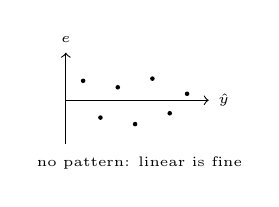
\begin{tikzpicture}[scale=0.55]
\draw[->] (0,0) -- (3.3,0) node[right,font=\tiny] {$\hat{y}$};
\draw[->] (0,-1.0) -- (0,1.1) node[above,font=\tiny] {$e$};
\fill (0.4,0.45) circle (1.5pt);
\fill (0.8,-0.4) circle (1.5pt);
\fill (1.2,0.3) circle (1.5pt);
\fill (1.6,-0.55) circle (1.5pt);
\fill (2.0,0.5) circle (1.5pt);
\fill (2.4,-0.3) circle (1.5pt);
\fill (2.8,0.15) circle (1.5pt);
\node[font=\tiny] at (1.7,-1.45) {no pattern: linear is fine};
\end{tikzpicture}}

\vspace{4pt}

\adjustbox{max width=\linewidth}{%
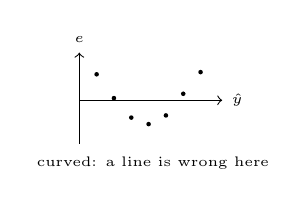
\begin{tikzpicture}[scale=0.55]
\draw[->] (0,0) -- (3.3,0) node[right,font=\tiny] {$\hat{y}$};
\draw[->] (0,-1.0) -- (0,1.1) node[above,font=\tiny] {$e$};
\fill (0.4,0.6) circle (1.5pt);
\fill (0.8,0.05) circle (1.5pt);
\fill (1.2,-0.4) circle (1.5pt);
\fill (1.6,-0.55) circle (1.5pt);
\fill (2.0,-0.35) circle (1.5pt);
\fill (2.4,0.15) circle (1.5pt);
\fill (2.8,0.65) circle (1.5pt);
\node[font=\tiny] at (1.7,-1.45) {curved: a line is wrong here};
\end{tikzpicture}}
\end{center}
\tiny{Residual against predicted value. The shape of the leftovers tells you whether a straight line was the right choice.}
\end{minipage}%
}%
\end{frame}

%%%%%%%%%%%%%%%%%%%%%%%%%%%%%%%%%%%%%%%%%%%%%%%%%%%
\begin{frame}[fragile]\frametitle{Quick Check: Multiple Regression}
\begin{block}{Think About It}
Fitted on its own, newspaper advertising has a clearly positive slope. Fitted alongside TV and radio, its slope drops to roughly zero. Nothing about the data changed between the two fits. So should the marketing team cut the newspaper budget, and what would you check first?
\end{block}
\end{frame}

%%%%%%%%%%%%%%%%%%%%%%%%%%%%%%%%%%%%%%%%%%%%%%%%%%%%%%%%%%%%%%%%%%%%%%%%%%%%%%%%%%
\begin{frame}[fragile]\frametitle{Quick Check: Multiple Regression}
\begin{block}{Answer}
Probably yes, but the reason matters more than the answer. The correlation matrix showed radio and newspaper spending move together at 0.35. Markets spending on newspaper were also spending on radio, so in the solo fit newspaper collected credit for radio's effect. Only the multiple regression, which holds the others fixed, separates them. What to check first is that correlation: a coefficient that changes sharply when you add other predictors is a signal that the predictors overlap, not that the data is faulty. Correlation between predictors is not proof that any one of them causes sales.
\end{block}
\end{frame}

%%%%%%%%%%%%%%%%%%%%%%%%%%%%%%%%%%%%%%%%%%%%%%%%%%%%%%%%%%%%%%%%%%%%%%%%%
%\begin{frame}[fragile]\frametitle{Answering questions using Regression Model}
%\begin{itemize}
%\item Question: How strong is the relationship between advertising budget and sales?
%\item Answer: RSE is 1,681 units while the mean value of the response is 14,022, indicating a percentage error of 12\%. Via $R^2$, the predictors explain almost 90\% of the variance in sales.
%\end{itemize}
%\end{frame}

%%%%%%%%%%%%%%%%%%%%%%%%%%%%%%%%%%%%%%%%%%%%%%%%%%%%%%%%%%%%%%%%%%%%%%%%%
%\begin{frame}[fragile]\frametitle{Answering questions using Regression Model}
%\begin{itemize}
%\item Question: Which media contribute to sales?
%\item Answer: Need to separate the effects of each medium. The p-values associated with TV and radio are low, while newspaper is not, suggesting that only TV and radio are related to sales.
%\end{itemize}
%\end{frame}
%
%%%%%%%%%%%%%%%%%%%%%%%%%%%%%%%%%%%%%%%%%%%%%%%%%%%%%%%%%%%%%%%%%%%%%%%%%
%\begin{frame}[fragile]\frametitle{Answering questions using Regression Model}
%\begin{itemize}
%\item Goal: What marketing plan for next year will result in high product sales?
%\item Question: How accurately can we estimate the effect of each medium on sales? For every dollar spent on advertising in a particular medium, by what amount will sales increase? How accurately can we predict this increase?
%\end{itemize}
%\end{frame}
%
%%%%%%%%%%%%%%%%%%%%%%%%%%%%%%%%%%%%%%%%%%%%%%%%%%%%%%%%%%%%%%%%%%%%%%%%%
%\begin{frame}[fragile]\frametitle{Answering questions using Regression Model}
%\begin{itemize}
%\item Answer: The 95\% confidence intervals for each medium are as follows: (0.043, 0.049) for TV, (0.172, 0.206) for radio, and (-0.013, 0.011) for newspaper. The confidence intervals for TV and radio are far from zero, providing evidence that these media are related to sales.
%\item Answer: Accuracy depends if we wish to predict an individual response (will use prediction interval), or the average response (use confidence interval). Prediction intervals are always wider because they account for the uncertainty associated with $\epsilon$, the irreducible error.
%\end{itemize}
%\end{frame}
%
%%%%%%%%%%%%%%%%%%%%%%%%%%%%%%%%%%%%%%%%%%%%%%%%%%%%%%%%%%%%%%%%%%%%%%%%%
%\begin{frame}[fragile]\frametitle{Answering questions using Regression Model}
%\begin{itemize}
%\item Goal: What marketing plan for next year will result in high product sales?
%\item Question: Is the relationship linear?
%
%\item Answer: Residual plots can be used in order to identify non-linearity. If the relationships are linear, then the residual plots should display no pattern.
%\end{itemize}
%\end{frame}


%%%%%%%%%%%%%%%%%%%%%%%%%%%%%%%%%%%%%%%%%%%%%%%%%%%%%%%%%%%%%%%%%%%%%%%%%
%\begin{frame}[fragile]\frametitle{Answering questions using Regression Model}
%\begin{itemize}
%\item Question: Is there any interaction effect? (called ``synergy'' in business). Example: spending 50k on TV ads + 50k on radio ads results in more sales than spending 100k on only TV
%\item Answer: The standard linear regression model assumes an additive relationship between the predictors and the response. The effect of each predictor on the response is unrelated to the values of the other predictors.
%\item Answer: The additive assumption may be unrealistic for certain datasets.
%\item Answer: Can extend linear model to include interaction term.
%
%\end{itemize}
%\end{frame}

%%%%%%%%%%%%%%%%%%%%%%%%%%%%%%%%%%%%%%%%%%%%%%%%%%%%%%%%%%%%%%%%%%%%%%%%%
%\begin{frame}[fragile]\frametitle{Back to the Car example...}
%\begin{center}
%
\includegraphics[width=\linewidth]{carex5}
%\end{center}
%\end{frame}



